%--------------------------------------------------------------------
\medskip
\subsection{Análisis funcional y diagrama de arquitectura de flujo de datos}
\label{02}
El sistema que se va a implementar consta de la siguiente funcionalidad:
\begin{itemize}
 \item Primero recogerá los datos de la fuente y aplicará técnicas ETL, para así obtener un conjunto de datos válido y preparado para permitir a los usuarios finales la posiblidad de realizar el análisis de las encuestas realizadas en todos los centros de sus clientes y poder hacer un seguimiento de los mismos.
 \item Para poder realizar el análisis, el sisteman proporcionará distintos tipos de gráficos, como por ejemplo, la evolución temporal de los resultados obtenidos en cada uno de los cuestionarios; también la posiblidad de saber en qué centro se obtienen los mejores/peores resultados, entre otros.
\end{itemize}

Así pues, en la Figura \ref{02-image} se muestra la arquitectura del flujo de datos. 
\begin{figure}[!th]
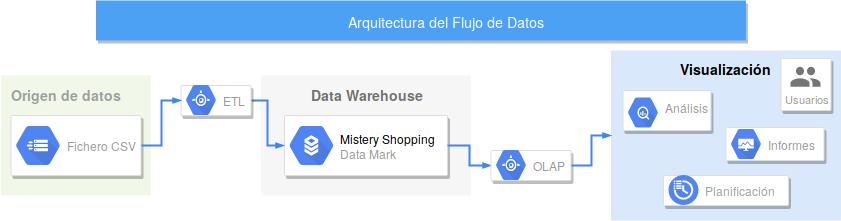
\includegraphics[scale=0.5]{02.png}
\centering
\caption{Arquitectura del flujo de datos.}
\label{02-image}
\end{figure}
